\documentclass[11pt]{article}

\usepackage{amsmath,amssymb,amsfonts}
\usepackage{booktabs}
\usepackage{graphicx}
\usepackage{hyperref}
\usepackage{tikz}
\usepackage{xcolor}
\usepackage[margin=1in]{geometry}
\usepackage[numbers,square,sort&compress]{natbib}
\usepackage[affil-it]{authblk}
\usepackage{lineno}
\linenumbers

\renewcommand{\arraystretch}{1.3}
\setlength{\abovetopsep}{6pt}

\title{Construct Validity for Cross-Context Consistency Scores:\\ Confound Tests Across 36,000 Drug, Genetic, and Morphological Perturbations}

\author{Elliot Tower}
\affil{\texttt{elliot@elliottower.ai}}

\date{}

\begin{document}
\maketitle

\begin{abstract}
\textbf{Background:}
Given thousands of profiled compounds and budget for dozens, a practitioner
ranks by a cross-context consistency score and follows up the top of the
list. Direction instability, which measures the angular consistency of a
perturbation's response across contexts---cell lines, cell types, or
imaging sites---produces such rankings.
Whether they survive correction for toxicity programs, off-target
consistency and universal-essential effects has not been tested.

\textbf{Results:}
We report eight pre-registered confound tests across 10{,}625 drug and
genetic perturbations in LINCS L1000 and Perturb-seq, with
Holm--Bonferroni correction within domain, and a morphological
feature-ablation sensitivity analysis in 24{,}992 JUMP-CP compounds.
The ranking is stable in aggregate: raw and corrected scores agree at
Spearman $\rho = 0.91$ in Perturb-seq and $\rho > 0.99$ in LINCS, and the
morphological ablation leaves the JUMP-CP ranking nearly unchanged
($\rho = 0.998$, $n = 24{,}992$). It is
not stable item by item: proteasome and spliceosome components move
660--900 positions of 1{,}676 under a correction whose global effect is
$\rho = 0.91$. The displacement is not noise. Phenotype projection
separates on-target from off-target consistency ($\rho = 0.376$ against
on-target genetic connectivity, versus $-0.043$ for the raw score; a
pre-registered CRISPRi convergent-validity check did not independently
confirm it), and separates compounds the raw score cannot: daunorubicin and MG-132 have
near-identical scores ($0.557$, $0.565$), but only daunorubicin's
consistency projects onto its annotated target. Essential-gene correction
inverts the predicted confound direction, with universal-essential
knockdowns diverging rather than converging across cell types ($d = 0.60$,
$p_{\text{perm}} < 10^{-4}$). Toxicity correction shifts scores by less
than $0.01$, refuting the predicted confound: cytotoxic compounds already
occupy the high-instability regime.

\textbf{Conclusions:}
Corrections do not change which perturbations rank highly; they identify
which highly-ranked perturbations move under correction. A score adequate
for population-level comparison is not adequate for a claim about any
single perturbation, and a high global correlation between raw
and corrected rankings is not evidence that the correction was
unnecessary.
\end{abstract}

\paragraph{Keywords:} construct validity, geometric perturbation scores, mechanistic claims, direction instability, LINCS L1000, Perturb-seq, Cell Painting, rank stability, pre-registration, Fr\'{e}chet variance, Grassmannian geodesic

\section{Background}

Geometric perturbation scores---metrics that quantify how a biological
system's response to a perturbation varies across experimental
contexts---rank drugs, genes, and compounds by mechanism conservation
across large-scale profiling datasets
\citep{lamb2006connectivity,subramanian2017next}. Direction instability,
one such score, measures the angular consistency of perturbation signatures
across cell lines: a drug whose transcriptomic response points in the same
direction regardless of cell type receives a low score, indicating conserved
mechanism \citep[preprint, under review;][]{tower2026drug}. Applied to
8{,}949 drugs in LINCS L1000,
direction instability produces biologically meaningful rankings: pan-HDAC
inhibitors achieve the lowest scores ($D = 0.49$--$0.55$), with a
selectivity gradient within the HDAC class (Figure~\ref{fig:hdac})
that tracks isoform specificity \citep[preprint, under
review;][]{tower2026atlas}.

\begin{figure}[t]
\centering
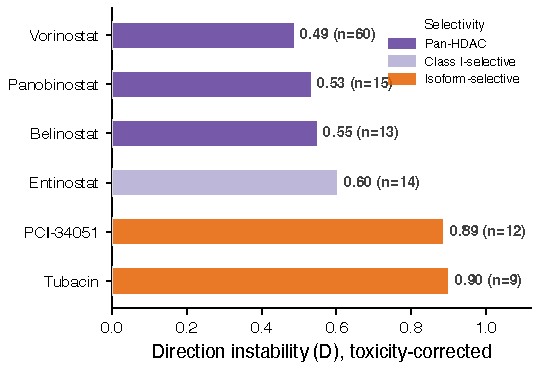
\includegraphics[width=0.85\linewidth]{figures/fig5_hdac.pdf}
\caption{%
\textbf{HDAC selectivity gradient: calibration panel for direction
instability.}
Toxicity-corrected direction instability for six HDAC inhibitors, grouped
by selectivity class. Pan-HDAC inhibitors \citep{bolden2006anticancer}
(vorinostat, panobinostat, belinostat) score $D = 0.49$--$0.55$;
Class~I-selective entinostat is intermediate ($D = 0.60$); the
isoform-selective inhibitors tubacin (HDAC6) and PCI-34051 (HDAC8)
\citep{balasubramanian2008hdac8} are highest ($D = 0.89$--$0.90$).
Selectivity is treated as three ordered categories rather than six ranks:
the pan-HDAC inhibitors differ in potency rather than in isoform breadth,
and the relative selectivity of tubacin and PCI-34051 is assay-dependent,
so neither pair supports an internal ordering. All 11 cross-category
comparisons are concordant (Kendall $\tau_b = 0.856$). Six compounds
admit no meaningful significance test, and none is reported; the panel
is a calibration reference, not an external validation. Plotted values are
read from \texttt{results/fig5\_hdac\_source/fig5\_hdac\_source.json}.}
\label{fig:hdac}
\end{figure}

Direction instability complements rather than replaces the
perturbation-quality and retrieval metrics already in use on these
datasets, and the estimands differ. The L1000 Transcriptional Activity
Score combines signature strength with replicate concordance to identify
transcriptionally active perturbations, so it registers the conjunction
that $D$ separates. Cell Painting percent-replicating asks whether
replicate profiles are more similar to each other than a null distribution
allows, and mean average precision scores retrieval of known replicate or
annotation groups. Each answers whether a perturbation produced a
reproducible measurable signal, or how well profiles retrieve a stated
label. $D$ answers a different question: given that a signal is present,
how much its direction changes across the contexts the analyst designates.
A perturbation can score well on activity and retrieval while carrying high
$D$, and the reverse holds for a weak but directionally stable
perturbation.

These rankings are consistent with the score carrying biological signal,
within the limits of the calibration panel of Figure~\ref{fig:hdac}.
They leave open a practical question: when can a practitioner trust a
geometric perturbation score for downstream decisions such as hit
prioritization, mechanism-of-action annotation, or cross-context
prediction? A score of $D = 0.55$ means signatures point in similar
directions across cell lines. It does not mean the drug acts through a
specific pathway or that the observation will replicate in a new context.

Three specific confounds threaten interpretation. The raw score cannot
distinguish on-target mechanism conservation from coherent off-target
programs. A drug scored from few cell lines may appear consistent due to
low Fr\'echet variance rather than genuine directional agreement. In
genetic perturbation screens, universal-essential knockdowns could inflate
or deflate cross-cell-type distances through a shared lethal-response
subspace. No systematic procedure exists for diagnosing which of these
threats a given score has survived
(cf.\ construct-validity frameworks in measurement theory
\citep{cronbach1955construct,messick1995validity}).

We formalize these threats through a validation framework
(Figure~\ref{fig:ladder}): a sequence of seven conditions that
progressively strengthen what a geometric perturbation score supports.
Each condition targets a specific confound. The ordering reflects logical
dependency: a reliable measurement (Condition~2) is prerequisite for
meaningful projection (Condition~5), and localized signal (Condition~4)
precedes phenotype alignment (Condition~5). Satisfying additional
conditions does not change the score; it narrows the set of confounds
that remain viable alternative explanations.

This paper tests whether these validation conditions matter empirically
across three perturbation domains: 8{,}949 LINCS L1000 drug compounds
\citep{subramanian2017next}, 1{,}676 Perturb-seq genetic knockdowns
\citep{replogle2022mapping}, and 24{,}992 JUMP-CP Cell Painting morphological
profiles \citep{chandrasekaran2023jump}. Direction instability serves as
the case study, but the procedure---define confounds, specify corrections,
pre-register predictions, test whether corrections reorganize rankings or
preserve them---applies to any geometric score measuring
perturbation-response consistency across contexts.

\section{Definitions and Notation}

\subsection{Direction instability}

For a drug tested in $K$ cell lines, let $\mathbf{s}_1, \ldots,
\mathbf{s}_K \in \mathbb{R}^{978}$ denote its consensus signature vectors.
Define unit-normalized signatures $\hat{\mathbf{s}}_i = \mathbf{s}_i /
\|\mathbf{s}_i\|_2$. Direction instability is:
\begin{equation}
  D = 1 - \frac{2}{K(K-1)} \sum_{i < j}
    \hat{\mathbf{s}}_i^\top \hat{\mathbf{s}}_j
  \label{eq:direction_instability}
\end{equation}
$D = 0$ when all signatures are collinear and $D = 1$ when they are
orthogonal on average, with $0 \leq D \leq K/(K-1)$, so the attainable
maximum is $2.000$ at $K = 2$ and $1.250$ at $K = 5$.

This quantity is not new. Writing $\bar{R} = \|\sum_i
\hat{\mathbf{s}}_i\|/K$ for the mean resultant length of the
unit-normalized signatures, the mean pairwise cosine in
Equation~\ref{eq:direction_instability} is $(K\bar{R}^2 - 1)/(K-1)$, which
is pairwise phase consistency (PPC), introduced by \citet{vinck2010ppc} as
a bias-free measure of synchronization---so $D = 1 - \mathrm{PPC}$. PPC was
designed for the property claimed here, separating consistency from
apparent strength due to sample size. What this study contributes is
therefore not the statistic but a construct-validity audit of it: which
confounds a cross-context consistency score survives, tested against
pre-registered predictions across three profiling modalities.
Cosine normalization removes the linear dependence on perturbation
magnitude (Figure~\ref{fig:dag}), under the assumption that signature
direction and magnitude are separable---that is, that the direction a
drug perturbs gene expression does not itself change with dose.
Direction instability measures only direction \citep{tower2026drug}.
Variance-based and estimation-based metrics conflate perturbation
strength with biological signal. The separability assumption is tested
empirically in the Discussion.

\begin{figure}[t]
\centering
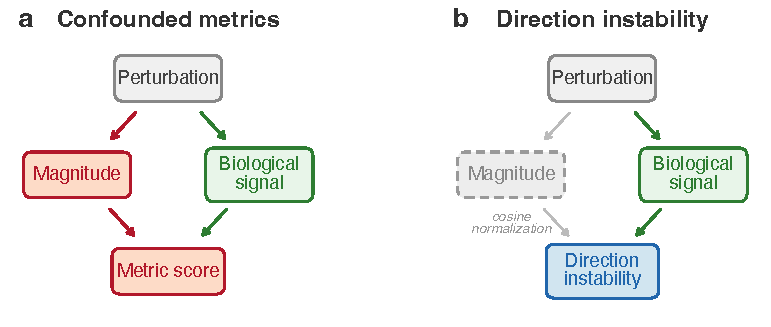
\includegraphics[width=\linewidth]{figures/fig1_dag_v3.pdf}
\caption{%
\textbf{Direction instability removes linear magnitude dependence.}
\textbf{(a)}~Confounded metrics (variance, subspace size) inherit effect
magnitude through a shared path, producing spurious associations between
perturbation strength and metric value.
\textbf{(b)}~Direction instability operates after cosine normalization,
which blocks the linear magnitude path under the assumption that signature
direction is independent of dose (separability). The observed
association between group variable and metric reflects biological signal
to the extent that this assumption holds.
An empirical test of separability (dose-direction stability across
1{,}445 drugs) is reported in the Discussion.}
\label{fig:dag}
\end{figure}

\subsection{Grassmannian geodesic distance in Perturb-seq}

Direction instability generalizes from vectors to subspaces. For a gene
knocked down in two cell types, let $U_1, U_2 \in \text{Gr}(k, d)$ denote
the top-$k$ PCA subspaces of the perturbation response in each cell type
($k$ = subspace dimension, $d$ = ambient dimension).
The Grassmannian geodesic distance $\delta(U_1, U_2) =
\|\boldsymbol{\theta}\|_2$, where $\boldsymbol{\theta}$ are the principal
angles between the subspaces, measures how much the perturbation response
\emph{rotates} across cell types. With $K = 2$ contexts, the pairwise
average in Eq.~\ref{eq:direction_instability} reduces to a single
comparison, and the estimand carries no Fr\'{e}chet variance or holonomy
information. We therefore do not compute direction instability as defined
in Eq.~\ref{eq:direction_instability} for Perturb-seq; we compute the
Grassmannian geodesic distance $\delta(U_1, U_2)$ between per-cell-type
response subspaces. This is a related but distinct geometric estimand, and
we label it as such throughout rather than presenting it as direction
instability at $K = 2$. Perturb-seq results are interpreted as a
subspace-rotation analysis, not a direct replication of the LINCS
vector-cosine analysis.

\subsection{Direction instability in Cell Painting morphological profiles}

Cell Painting \citep{bray2016cell,chandrasekaran2023jump} measures 3{,}180 morphological
features per well across five fluorescent channels. JUMP-CP
profiles 116{,}000 compounds across 10 imaging sources. Direction
instability applies directly: each compound's morphological signature in a
given source is a vector in $\mathbb{R}^{3180}$, and $D$ measures angular
consistency across sources. A JUMP-CP source is a partner imaging site
rather than a distinct cell type, so $D$ computed over sources indexes
cross-site technical reproducibility rather than context-dependence across
cell types. The JUMP-CP result is reported on that basis throughout. A frozen block of
252 features (7.9\% of the space) covers size and shape across compartments
together with DNA- and mitochondria-channel intensity, granularity and
radial distribution. The ablation removes that block and recomputes
direction instability. The block is an author-defined morphological feature
family rather than a validated cell-health signature; published cell-health
work defines phenotypic readouts and models predicting them rather than a
corresponding set of CellProfiler columns.

\subsection{The validity problem}

Consider two drugs with identical direction instability, $D \approx 0.56$
(mechanism-conserving regime):

\begin{itemize}
  \item \textbf{Drug A} is a topoisomerase~II inhibitor. Its conserved
    direction aligns with its target gene's knockdown
    signature---phenotype-projected instability is high. The consistency comes
    from on-target DNA-damage signaling.
  \item \textbf{Drug B} is a proteasome inhibitor. Its conserved direction
    does \emph{not} align with its annotated target subunit's knockdown
    signature---phenotype-projected instability is near zero. The consistency
    comes from broad proteostasis disruption shared across cell types.
\end{itemize}

Both achieve $D \approx 0.56$. Both pass the raw metric equally. Phenotype
projection (Condition~5 of the validation framework) distinguishes them: Drug~A's
consistency is mechanistically on-target; Drug~B's is not. The distinction
matters for downstream decisions: Drug~A is a strong candidate for
mechanism-based follow-up; Drug~B requires additional investigation to
identify what program drives its consistency before any mechanistic claim
is supported. A concrete instance of this scenario (daunorubicin vs.\
MG-132) appears in the Discussion.

\subsection{The validation framework}

The validation framework defines seven conditions for geometric
perturbation scores (Figure~\ref{fig:ladder}), ordered by logical
dependency rather than by evidence strength:

\begin{enumerate}
  \item \textbf{Process view declared.} What constitutes a ``context''?
  \item \textbf{Reliable vector field.} Adequate signal-to-noise for
    direction to be meaningful.
  \item \textbf{Perturbation estimable.} Effect isolated from background.
  \item \textbf{Localized to biology.} Instability concentrates in
    pathway-relevant genes.
  \item \textbf{Phenotype-aligned.} Conservation direction matches a
    known target pathway.
  \item \textbf{Transports across contexts.} Score replicates in held-out
    contexts (low Fr\'echet variance).
  \item \textbf{Predicts holdout.} Metric predicts an external outcome
    in new data.
\end{enumerate}

Conditions 1--3 are satisfied by design in our datasets and are not tested
further. Conditions 4--6 are tested empirically.
Condition~7 (holdout prediction in a genuinely new dataset) is not tested:
Experiment~5's leave-one-cell-line-out cross-validation tests Condition~6
(transport within LINCS), not generalization to an independent dataset.
A Condition~7 test would require predicting compound activity in a dataset
collected independently of LINCS---such as a proprietary pharma screen
or a future LINCS phase---using only validation-framework scores computed
from the current data.

\begin{figure}[t]
\centering
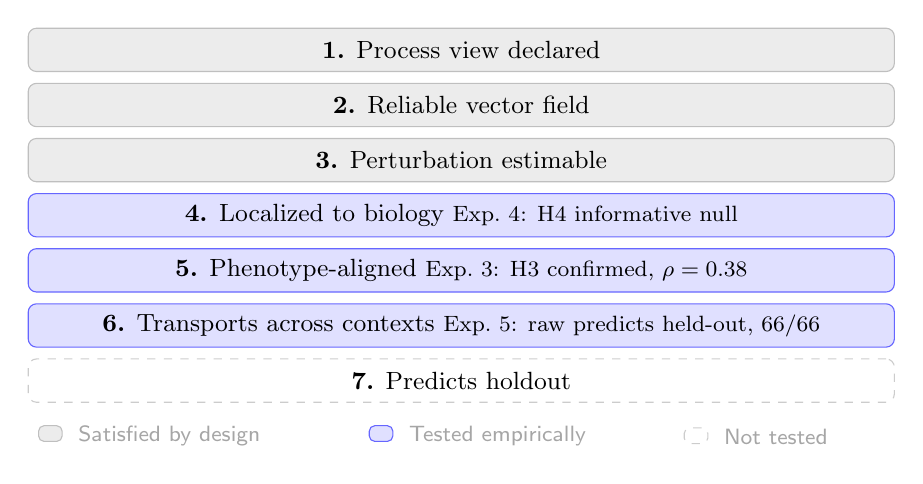
\begin{tikzpicture}[
  condition/.style={draw, rounded corners=3pt, minimum width=11cm, minimum height=0.55cm, font=\small},
  satisfied/.style={condition, fill=gray!15, draw=gray!50},
  tested/.style={condition, fill=blue!12, draw=blue!60},
  untested/.style={condition, fill=white, draw=gray!40, dashed},
  label/.style={font=\footnotesize\sffamily, text=gray!70},
]
\node[untested]  at (0, 0.0) {\textbf{7.} Predicts holdout};
\node[tested]    at (0, 0.7) {\textbf{6.} Transports across contexts \hfill \textnormal{\footnotesize Exp.~5: raw predicts held-out, 66/66}};
\node[tested]    at (0, 1.4) {\textbf{5.} Phenotype-aligned \hfill \textnormal{\footnotesize Exp.~3: H3 confirmed, $\rho = 0.38$}};
\node[tested]    at (0, 2.1) {\textbf{4.} Localized to biology \hfill \textnormal{\footnotesize Exp.~4: H4 informative null}};
\node[satisfied] at (0, 2.8) {\textbf{3.} Perturbation estimable};
\node[satisfied] at (0, 3.5) {\textbf{2.} Reliable vector field};
\node[satisfied] at (0, 4.2) {\textbf{1.} Process view declared};
% Legend
\node[label, anchor=west] at (-5.5, -0.7) {%
  \tikz\draw[fill=gray!15, draw=gray!50, rounded corners=2pt] (0,0) rectangle (0.3,0.2);
  ~Satisfied by design};
\node[label, anchor=west] at (-1.3, -0.7) {%
  \tikz\draw[fill=blue!12, draw=blue!60, rounded corners=2pt] (0,0) rectangle (0.3,0.2);
  ~Tested empirically};
\node[label, anchor=west] at (2.7, -0.7) {%
  \tikz\draw[fill=white, draw=gray!40, dashed, rounded corners=2pt] (0,0) rectangle (0.3,0.2);
  ~Not tested};
\end{tikzpicture}
\caption{%
\textbf{The validation framework.}
Seven conditions progress from measurement prerequisites (1--3)
through empirically tested validation conditions (4--6) to external
prediction (7). Each condition targets a specific confound.
Conditions~4--6 are tested across three domains (LINCS L1000, Perturb-seq,
JUMP-CP); result summaries are shown at right. Satisfying additional
conditions does not change the direction-instability score---it narrows
the set of confounds that remain viable.}
\label{fig:ladder}
\end{figure}

\section{Related work}

\paragraph{Validation frameworks for computational scores.}
Recent work has formalized validation procedures for computational scores:
construct-validity frameworks for ML benchmarks
\citep{freiesleben2025benchmarking,watson2025measuring}, the SBB
principles for perturbation-prediction models \citep{sbb2026principles},
and the classical construct-validity tradition in psychometrics
\citep{cronbach1955construct,messick1995validity}. Our validation
framework draws on these precedents, instantiating them for geometric
perturbation scores. A mapping between the framework's conditions and
Messick's six validity facets appears in Supplementary Table~S1.

\paragraph{Perturbation biology.}
CERES \citep{meyers2017ceres} corrects copy-number artifacts in CRISPR
screens; integrated Broad--Sanger analyses \citep{pacini2021integrated}
document cross-study divergence. These corrections operate on
dependency-score magnitudes; our contribution is orthogonal, correcting
subspace geometry and showing that rank-preserving corrections carry
diagnostic value. The Connectivity Map framework
\citep{subramanian2017next,lamb2006connectivity} and subsequent metric
evaluations \citep{li2020comprehensive} establish the
transcriptomic-similarity scoring approach that direction instability extends.
LEMUR \citep{ahlmanneltze2025lemur} performs multivariate regression on
Grassmann manifolds for multi-condition Perturb-seq; our Experiment~7 uses
a simpler Grassmannian geodesic distance. Raju's geometric coherence
framework \citep{raju2026shesha} applies related angular measures to
single-cell CRISPR perturbations; our work differs in testing construct
validity of such scores rather than using them directly for prediction.
Pharmacogenomic interaction landscapes \citep{iorio2018unsupervised}
and retrieval-based profile evaluation \citep{kalinin2025versatile}
provide complementary perspectives on cross-study consistency.

\paragraph{Metric evaluation in perturbation biology.}
Prior work has benchmarked connectivity and signature-similarity metrics
for consistency and predictive value
\citep{subramanian2017next,li2020comprehensive,napolitano2021reconciling},
validation
frameworks have been proposed for ML benchmarks and computational scores
\citep{freiesleben2025benchmarking,watson2025measuring}; and recent work
has shown that simple linear baselines match deep-learning perturbation
predictors \citep{ahlmanneltze2025baseline}, while neural optimal
transport \citep{bunne2023cellot} offers an alternative geometric
approach to perturbation response modeling. These efforts
evaluate \emph{whether} a metric predicts a downstream label. Our
contribution is orthogonal: we test \emph{which confounds a given score
has survived}---treating validation as a graded, condition-dependent
diagnostic rather than a single predictive-accuracy number---and
identify where those conditions affect interpretation across three
perturbation modalities. We are not aware of a comparable
condition-by-condition validation applied to an unsupervised geometric
perturbation score with pre-registered decision criteria.

\section{Methods}

\subsection{Data}

Perturbation signatures were drawn from LINCS L1000 Phase~I (GEO accession
GSE92742; $\sim$1.3 million profiles across $\sim$50 cell lines),
using Level~5 replicate-collapsed z-scores across 978 landmark genes
\citep{subramanian2017next,keenan2018library}. Of 77 cell lines in Phase~I,
approximately 50 contribute sufficient compound coverage for direction
instability computation. We retained 8{,}949
small-molecule perturbagens tested in $\geq5$ cell lines.

Perturb-seq data derive from \citet{replogle2022mapping}: genome-scale
CRISPRi knockdowns in K562 and RPE1 cells. We extracted 1{,}676 genes
with $\geq$30 perturbed cells in both cell types, computed per-gene
expression responses over 2{,}073 highly variable genes, and fitted
$k = 5$ PCA subspaces per gene per cell type (of these, 1{,}567 have
matching DepMap Chronos labels for HP3; all 1{,}676 are used for HP1).
Both screens target DepMap-essential genes; 85\% of RPE1 targets overlap
with K562 targets. Essentiality labels derive from DepMap Chronos scores
\citep{dempster2021chronos}: 855 genes with Chronos $< -0.5$ in both
K562 and RPE1 were classified as universal-essential; the remaining 712
are sub-threshold and serve as the comparison group. A label-permutation
null (10{,}000 permutations) tested whether the observed group difference
exceeds background K562/RPE1 divergence.

JUMP-CP Cell Painting profiles derive from the Cell Painting Gallery
\citep{chandrasekaran2023jump}: 24{,}992 compounds tested in $\geq$5
imaging sources after filtering (78.4\% attrition from the 115{,}729
total; the majority of compounds appear in fewer than 5 sources,
making direction instability---which requires multiple
contexts---undefined for them), with eight plate-level control compounds
excluded. The ablated block (252 features matching Area, Compactness,
Eccentricity, Extent, FormFactor, Solidity, DNA/Mito Intensity,
Granularity and Radial Distribution) was resolved once against the release
schema and hashed; ablated direction instability was computed
on the remaining 2{,}437 features.

Following pre-registration principles \citep{nosek2018preregistration},
all scoring functions and drug lists were committed before any real LINCS
signatures were analyzed (initial freeze: commit \texttt{8d74bd0}).
Perturb-seq hypotheses and extended drug hypotheses (H5-full,
H3-CRISPRi) were pre-registered before the correction analysis
(commit \texttt{f3c88ed}, tag \texttt{prereg-extended-psb}, timestamped
2026-07-08T11:56:58--04:00, preceding experiment results committed at
14:42--04:00). The dose-direction separability test
(Section~6.2) was pre-registered in commit \texttt{5bb6080} before
execution. The repository was public at the time of all freezes.\footnote{Code, pre-registration, deviation log, and all
experimental scripts:
\url{https://github.com/elliottower/direction-instability-drug-validity}.
LINCS data: GEO GSE92742; Perturb-seq: \citet{replogle2022mapping};
JUMP-CP: \citet{chandrasekaran2023jump}; DepMap: \citet{dempster2021chronos}.}

\paragraph{Reporting guidelines.}
No existing reporting guideline (such as TRIPOD for clinical prediction models)
directly governs a validation study of an unsupervised geometric score.
We adopt TRIPOD's spirit where applicable---pre-specified analysis plan,
frozen thresholds, complete reporting of all pre-registered hypotheses
including nulls---and note deviations in Table~\ref{tab:deviations}.
We omit items (such as patient-level calibration and outcome incidence) that
do not apply to a non-clinical perturbation-screen setting.

\begin{table}[t]
\centering
\caption{Deviation log. All departures from the pre-registered plan, with
rationale and timing. Full detail in \texttt{DEVIATION\_LOG.md},
commit-linked.}
\label{tab:deviations}
\small
\begin{tabular}{cp{3.2cm}p{3.2cm}p{3.8cm}l}
\toprule
\# & Pre-registered & Actual & Why & When \\
\midrule
1 & Hypotheses frozen; gene-set method unspecified &
  Gene-set method declared in extended pre-reg &
  Original freeze omitted gene-set construction parameters for H3/H4/H5 &
  Pre-analysis \\
2 & H5: $\geq$4/5 folds win &
  Threshold adjusts to $\lceil 0.8 n \rceil$ if $<$5 valid folds &
  Maintains 80\% win rate when rare cell lines have too few drugs;
  not triggered in practice (71 cell lines) &
  Pre-analysis \\
3 & H3 and H4 treated as independent &
  Shared shRNA-consensus dependency documented &
  Both derive from the same genetic perturbation object; not independent tests &
  Pre-analysis \\
4 & Original H5: 5 alphabetical folds &
  Full 66-fold leave-one-out with Wilcoxon co-primary &
  Extended pre-reg (commit \texttt{f3c88ed}) replaces original &
  Pre-analysis \\
5 & H3-CRISPRi: three-outcome decision tree &
  Outcome~(c) realized ($\rho = -0.12$) &
  Followed frozen decision tree; K562-only confound explanation pre-registered &
  Post-analysis \\
6 & H5 win test $\rho_{\text{TS}} > \rho_{\text{raw}}$ &
  Reported as not confirmed; predictive strength compared on $|\rho|$ &
  The registered test compares signed correlations between
  oppositely-oriented statistics, so its criterion is satisfiable by
  orientation rather than by prediction; the registration omitted an
  orientation convention &
  Post-analysis \\
\bottomrule
\end{tabular}
\end{table}

We treat the five LINCS hypotheses (H1--H5) as one test family and the
three Perturb-seq hypotheses (HP1--HP3) as a second. The separation
reflects genuine independence: the two domains use different experimental
systems (50+ cell lines vs.\ two specific lines), different perturbation types
(small molecules vs.\ CRISPRi), different geometric estimands (vector
cosines in $\mathbb{R}^{978}$ vs.\ Grassmannian geodesics in Gr$(5, 2073)$),
and share no data or parameters. A single family across all eight hypotheses
would be more conservative; we consider it overly so given the absence of
any shared data or analytic dependence between domains. The choice is
immaterial for the confirmed result: H3 ($p < 10^{-27}$) survives
Holm--Bonferroni correction even under a single 8-hypothesis family. Experiment~8
enters no multiplicity family: it tests no registered hypothesis, and its
context axis is the imaging source rather than a biological one. After Holm--Bonferroni
correction within the drug family, H3 ($p < 10^{-27}$) survives at
$\alpha = 0.05$; H2 ($p = 0.28$), H4 (gap $= 0.018$) and H5 (10 of 66
folds) do not;
H1's criterion-pass is an artifact.
HP3 registered no pass/fail threshold, so it enters no multiplicity
family and is reported descriptively.

\subsection{Phenotype-projected instability (Experiment 3)}

For each drug with an annotated target gene (Drug Repurposing Hub
\citep{corsello2017drug}, 1{,}551 drugs), the ``on-target direction'' is the consensus shRNA
knockdown signature of that target gene in LINCS L1000 (4{,}369 genes
eligible, $\geq$3 hairpins each, consensus averaged across up to 20 cell lines).
Phenotype projection projects the instability vector onto this
on-target direction. On-target enrichment is defined as $\cos^2(\bar{\mathbf{s}}_{\text{drug}},\,
\bar{\mathbf{s}}_{\text{shRNA}})$: the squared cosine between each drug's
mean signature and its target gene's shRNA consensus, measuring how much
of the drug's transcriptomic effect aligns with the genetic perturbation of
its annotated target.

shRNA signatures have well-documented off-target effects
\citep{smith2017evaluation}, which add noise to the on-target direction
and attenuate the observed correlation: the true on-target association is
likely stronger than the measured $\rho = 0.38$.
The shRNA consensus averages across up to 20 cell lines, producing a
cell-type-agnostic on-target direction at the cost of off-target
contamination. Similarly, Drug Repurposing Hub target annotations carry
noise from multi-target compounds and legacy assignments; misannotation
further attenuates the correlation. Polypharmacology compounds this:
drugs with strong secondary targets may show phenotype projection onto the
primary target even when cross-cell-line consistency is driven by a
secondary mechanism, a confound that single-target annotations cannot
resolve. A convergent-validity
check using CRISPRi signatures (single cell type, cleaner
loss-of-function but cell-type-specific) is reported in the Results.

The pre-registered prediction (H3) required Spearman $|\rho| > 0.3$ between
phenotype-projected instability and on-target enrichment, and $|\rho| < 0.15$
for raw direction instability versus the same enrichment.

\subsection{Variance-regularized direction instability (Experiment 5)}

Transport-stable (TS) direction instability regularizes the raw score by
subtracting a penalty proportional to the Fr\'{e}chet variance of the
signature directions across contexts:
\begin{equation}
  \text{TS} = D - \lambda \cdot \text{Var}_{\text{Fr\'echet}}
  \label{eq:ts}
\end{equation}
where $\text{Var}_{\text{Fr\'echet}} = \frac{1}{K}\sum_i
\arccos^2(\hat{\mathbf{s}}_i^\top \bar{\mathbf{s}})$ and
$\bar{\mathbf{s}}$ is the Fr\'echet mean direction. The subtraction downweights drugs whose apparent directional consistency
is driven by a small number of tightly clustered contexts rather than by
genuine mechanism conservation. The alternative (a ratio) would be
undefined when $\text{Var}_{\text{Fr\'echet}} = 0$ and would amplify
noise for highly consistent drugs. The penalty weight $\lambda$ was fixed
at the value from \citet{tower2026drug} and was not optimized for this
evaluation; a sensitivity analysis across a 20-fold range of $\lambda$
values is reported in Section~\ref{sec:exp5}.

We evaluate via leave-one-cell-line-out cross-validation over all cell
lines with $\geq 20$ eligible drugs after excluding the held-out cell line
(66 valid folds out of 71 total; 5 excluded for insufficient drug count).
A preliminary 5-fold analysis using alphabetically-selected cell lines
(A375, A549, A673, AGS, ASC) established the rare/common regime distinction
with permutation nulls; the full leave-one-out extends this to all cell
lines and adds Wilcoxon signed-rank as a co-primary criterion.

The pre-registered prediction (H5) required TS to outpredict raw direction instability
in $\geq 80\%$ of valid folds (co-primary~1), with Wilcoxon signed-rank on
per-fold $\Delta\rho$ rejecting $H_0$: median $\leq 0$ at $\alpha = 0.05$
(co-primary~2).

\subsection{Essential-gene correction on Perturb-seq (Experiment 7)}

We computed the Fr\'echet mean subspace of the 855 essential-gene
perturbation responses (separately in K562 and RPE1) via iterative
projection on Gr$(5, 2073)$ (100 iterations, convergence to
$\Delta < 10^{-6}$ in Grassmannian distance; the result is insensitive
to initialization because the essential-gene subspaces cluster tightly).
We then projected this essential-response subspace out of each gene's
response subspace, re-orthogonalized, and recomputed geodesic distances.

Two pre-registered predictions were tested.
HP1 required Spearman $\rho$ between raw and corrected distances below
0.70 (ranking-disruptive, denoted ``bites'') or $\geq 0.83$
(ranking-preserving, denoted ``doesn't bite''). We use these shorthand
terms throughout: a correction ``bites'' when it reorganizes the
population ranking ($\rho < 0.70$) and ``doesn't bite'' when it
preserves it ($\rho \geq 0.83$). The ranking-preserving threshold of
0.83 was calibrated to the within-class ordering of the HDAC selectivity
gradient (Figure~\ref{fig:hdac}) and is retained as the pre-registered
decision rule. It rests on six compounds and is not offered as a generally
validated cutoff; every domain-level classification is unchanged at 0.89
or 0.90, since the observed correlations are 0.91 and $>$0.99. The ranking-disruptive threshold of 0.70 was set as a
round-number boundary below which more than half the variance is
unexplained ($R^2 < 0.49$), following the companion paper
\citep{tower2026drug}. Values between 0.70 and 0.83 would require
further analysis to interpret.
HP3 predicted that universal-essential knockdowns produce higher geodesic
distances than non-essential knockdowns (Cohen's $d > 0$). The registration
records this hypothesis as descriptive, with no pass/fail threshold, and
discloses that the direction had been observed on a preliminary run before
the plan was frozen. HP3 therefore registers the robustness of an effect
already seen, not its direction, and is reported as directional support
rather than as a confirmed prediction.

\subsection{Morphological feature ablation on JUMP-CP (Experiment 8)}

Experiment~8 is a sensitivity analysis and carries no registered hypothesis.
It asks whether the compound ranking produced by $D$ survives deletion of a
structured block of morphological coordinates. The 252 ablated features are
7.9\% of the space, against 4.2\% (41/978) for the LINCS toxicity gene set.

Deleting 252 of 3{,}180 coordinates perturbs a cosine whatever the
coordinates are, so the block is compared against 200 ablations of randomly
selected feature sets of the same size rather than against no deletion.
Robustness is assessed by dropping each imaging source in turn and by
summarizing absolute percentile-rank shifts. Eight compounds present on at
least half of all eligible COMPOUND plates are plate-level controls rather
than screened compounds and are excluded before any ranking is formed.

The 0.70 and 0.83 thresholds are reported for continuity with the registered
domains. They do not discriminate here: random deletion of the same number of
features gives a median $\rho$ of $0.9998$, so any ablation of this size
clears $0.83$.

\subsection{Supplementary experiments}

Three additional drug-domain experiments are reported in Supplementary
Experiments. \textbf{Experiment~1}
(H1, toxicity correction) tests whether cytotoxic drugs masquerade as
mechanism-conserving. \textbf{Experiment~2} (H2, broad-mechanism drugs)
tests whether broad-target therapeutics fall below the population median.
\textbf{Experiment~4} (H4, localization score) tests whether gene-set
restriction improves MOA prediction. HP2 (GO pathway prediction from
corrected Perturb-seq distances) is also in Supplementary Experiments.

\section{Results}

\subsection{Pre-registered scorecard}

Table~\ref{tab:scorecard} summarizes the eight pre-registered hypotheses,
with the JUMP-CP sensitivity analysis listed separately beneath them.
One of five drug hypotheses survives Holm--Bonferroni correction (H3);
H2 meets its pre-registered criterion but does not survive multiplicity
correction; H1 is refuted with an artifact criterion-pass; H4 is an
informative null.
In the Perturb-seq domain, HP3 is confirmed; HP1 shows the correction
``doesn't bite'' at the population level; HP2 is a null. Experiment~8 carries
no registered hypothesis and appears in the table as a sensitivity analysis:
the morphological ablation preserves the JUMP-CP ranking, and the registered
threshold does not separate that from deleting an equal number of arbitrary
coordinates.

\begin{table}[t]
\centering
\caption{Pre-registered scorecard.
\emph{Criterion} = did the result meet the frozen pre-registered
threshold?
\emph{Holm} = does it survive Holm--Bonferroni correction within its
domain family ($\alpha = 0.05$)?
\emph{Status} = the interpretive status after both checks.
H1 and H2 dissociate: both meet their pre-registered criteria, yet H1
is refuted (criterion-pass is an artifact) and H2 does not survive
multiplicity correction.
Result details for starred entries appear in Section~5.6.}
\label{tab:scorecard}
\small
\begin{tabular}{@{}lp{2.7cm}p{3.0cm}p{1.7cm}cp{3.3cm}@{}}
\toprule
 & Prediction & Result & Criterion & Holm & Status \\
\midrule
H1$^\star$ & Toxicity reclassifies & $\Delta < 0.01$ & Met (artifact) & --- & \textbf{Refuted}---artifact of pre-existing high instability \\
H2$^\star$ & Broad drugs below median & 7/10 below & Met & No & \textbf{Suggestive}---does not survive multiplicity \\
H3 & $|\rho_{\text{proj}}| > 0.3$ & $\rho = 0.376$ & Met & Yes & \textbf{Confirmed} \\
H4$^\star$ & AUROC gap $> 0.05$ & Gap $= 0.018$ & Not met & No & \textbf{Informative null}---domain-dependent \\
H5 & TS wins $\geq$80\% folds & 10/66 on $|\rho|$; raw $\rho=-0.602$ in 66/66 & Not met & --- & \textbf{Not confirmed} \\
\midrule
HP1 & Correction bites ($\rho < 0.70$) & $\rho = 0.91$ & Not met & --- & \textbf{Doesn't bite} \\
HP2$^\star$ & GO prediction improves & $\Delta\rho = -0.02$ & Not met & --- & \textbf{Doesn't bite} \\
HP3 & Essential $d > 0$ (descriptive) & $d = 0.60$ & --- & --- & \textbf{Directional support}---inverts the predicted confound \\
\midrule
\multicolumn{6}{l}{\emph{Unregistered sensitivity analysis}}\\
Exp.~8 & --- & $\rho = 0.998$, $n = 24{,}992$ & --- & --- & \textbf{Ranking preserved} \\
\bottomrule
\end{tabular}
\end{table}

\subsection{Held-out cell-line agreement (Experiment 5)}
\label{sec:exp5}

H5 is not confirmed. The registered criterion was met (66/66 folds) but
is uninformative: direction instability measures inconsistency while
held-out cosine measures agreement, so a working score must correlate
negatively, and the transport-stable variant subtracts a term that
reverses that sign. Compared on predictive strength, the variant wins 10
of 66 folds and loses in the two largest ($|\rho| = 0.155$ against
$0.480$ for A375; $0.201$ against $0.494$ for A549). Five cell lines were
excluded for having $< 20$ eligible drugs.

The comparison establishes a property of the raw score instead. Direction
instability computed on the retained cell lines predicts whether the
held-out cell line agrees with their consensus: mean Spearman
$\rho = -0.602$ (range $[-0.784, -0.223]$), correctly signed in all 66
folds. A drug whose training signatures disagree with one another also
disagrees with a cell line it has not been measured in.
The advantage is drug-specific rather than algebraic. Under a
variance-preserving permutation null on the preliminary five-fold analysis,
held-out \emph{signatures} are shuffled across drugs while training data
remain fixed, and held-out cosines are recomputed against each drug's
original consensus. Across 1{,}000 permutations the observed prediction
falls entirely outside the null distribution
($p_{\text{perm}} < 10^{-3}$).

Prediction is strongest in cell lines with many profiled drugs and weakest
in rare ones, where removing a single cell line substantially changes the
consensus direction. Across the 66 folds $\rho$ ranges from $-0.784$ to
$-0.223$, and the folds with the fewest eligible drugs sit at the weak end
of that range. How many contexts a ranking requires before it reproduces is
the subject of separate work.


\subsection{On-target and off-target separation (Experiment 3)}

Among 795 drugs with annotated targets and matched shRNA consensus signatures,
phenotype-projected instability correlates with on-target enrichment at Spearman
$\rho = 0.376$ ($p = 4.8 \times 10^{-28}$). Raw direction instability shows no correlation
($\rho = -0.043$, $p = 0.22$). Both pre-registered criteria are satisfied.

H3 confirms Condition~5 of the validation framework. Raw direction instability
measures whether a drug's signatures point in consistent directions, but
this consistency could arise from any coherent program. Projecting onto the
genetic perturbation direction of the annotated target isolates the
mechanistically relevant component. The near-zero raw correlation shows
that global instability carries no on-target information; the strong
projected correlation shows that the on-target projection recovers it.

The gene-set construction avoids researcher degrees of freedom: the shRNA
consensus is an empirical object from the same LINCS platform,
requiring no pathway database selection. H3 and H4 share this shRNA
dependency (documented in DEVIATION\_LOG.md entry~3) and are not
independent tests. The phenotype-projected instability is applicable only
to drugs with target annotations---1{,}551 of 8{,}949 (17\%). For the
remaining 82\% of drugs with unknown targets, the validation framework
provides other conditions (transport stability, localization) that do not
require target annotations.

As a pre-registered convergent-validity check, we recomputed
phenotype-projected instability using CRISPRi loss-of-function signatures
\citep{replogle2022mapping} as the on-target
direction. The projected-instability correlation with on-target enrichment
did not reach significance (Spearman $\rho = -0.12$, $p = 0.16$,
$n = 131$), corresponding to pre-registered outcome~(c). On the
114-drug matched subset (drugs with both ground truths), shRNA
projection yields $\rho = 0.42$ while CRISPRi projection yields
$\rho = -0.14$, confirming that the ground-truth source---not the
drug set---drives the difference.

The pre-registered secondary criterion points to the likely cause: raw
instability correlated positively with CRISPRi enrichment
($\rho = +0.27$, $p = 0.002$) while projected instability did not---the
reverse of the shRNA pattern. This reversal is consistent with the
pre-registered K562-only confound: CRISPRi signatures derive from a
single hematopoietic cell type, so the CRISPRi ``on-target direction''
captures cell-type-specific effects rather than cross-context
mechanism---a confound that multi-cell-line shRNA consensus avoids by
averaging across ${\sim}20$ cell lines. One plausible explanation for
the positive raw-instability/CRISPRi correlation, which we did not test
directly, is that K562 expresses many drug targets at high levels,
producing spurious alignment between raw instability and K562-specific
signatures.

CRISPRi does not provide independent convergent validity for H3. The
shRNA-based result stands on its original evidence rather than being
reinforced. An alternative concern is that the H3 correlation is
partly tautological: both drug signatures and shRNA ground-truth
signatures derive from the same LINCS platform and largely overlapping
cell lines, so shared platform-specific variance could inflate the
association. The near-zero \emph{raw}-instability correlation
($\rho = -0.04$) argues against this: if platform sharing drove the
result, raw direction instability should also correlate with shRNA enrichment, since
it uses the same signatures. The correlation emerges only after
phenotype projection, suggesting it reflects on-target alignment
rather than shared platform noise.

\paragraph{HDAC-removal sensitivity.}
Pan-HDAC inhibitors are the calibration standard for direction instability
(Figure~\ref{fig:hdac}), so the H3 correlation could be driven by this
single drug class. To test this, we removed all 20 HDAC-targeting drugs
(spanning HDAC1, HDAC2, and HDAC6 targets; full list in Supplementary Experiments)
and recomputed the phenotype-projected correlation. The result is
essentially unchanged: $\rho = 0.3759$ ($n = 775$,
$p = 2.0 \times 10^{-27}$), compared with $\rho = 0.3756$ on the full
795-drug set ($\Delta\rho = 3 \times 10^{-4}$). A synonym check for ``histone
deacetylase,'' ``class~I HDAC,'' ``pan-HDAC,'' and ``sirtuin'' confirmed
no drugs were missed by the primary filter.

Removing the 20 drugs with lowest raw direction instability (most directionally
consistent regardless of class) also preserves the correlation
($\rho = 0.387$, $p = 4.8 \times 10^{-29}$). Removing the 20 drugs with
highest projected instability---a direct test of whether a handful of
phenotype-aligned outliers carry the signal---yields $\rho = 0.350$
($p = 9.8 \times 10^{-24}$). All three removal analyses exceed the
pre-registered threshold of $\rho > 0.20$. Bootstrap 95\% CI on the full
set is $[0.315, 0.433]$, excluding zero. The H3 correlation is broad-based,
not driven by HDAC inhibitors or a small number of extreme drugs.

\subsection{Essential-gene correction (Experiment 7)}

Universal-essential knockdowns have \emph{higher} Grassmannian geodesic
distances than non-essential knockdowns (mean 2.80 vs.\ 2.67, Cohen's $d =
+0.60$, Mann--Whitney $p < 10^{-33}$; $n = 1{,}567$ genes with both
geodesic distances and DepMap labels, of which 855 universal-essential and
712 sub-threshold). Cohen's $d = 0.60$ is a medium effect---the
distributions overlap substantially, and individual genes span the full
range in both groups. The finding is that the \emph{group means} differ
in the opposite direction from the predicted confound, not that essentiality
status determines geodesic distance.

Essential genes do not produce a shared response across cell types; they
\emph{diverge}---the same gene's lethal disruption manifests through
different transcriptomic programs in K562 and RPE1
(Figure~\ref{fig:cross_domain}). This is consistent with cell-line-specific
essentiality effects documented in CERES \citep{meyers2017ceres} and
integrated Broad--Sanger analyses \citep{pacini2021integrated}: the
functional consequences of losing a core-machinery gene depend on
the cell's lineage and metabolic context.

A label-permutation null (shuffling essential/non-essential labels across
the 1{,}567 genes, 10{,}000 permutations) confirms that this divergence
exceeds background K562/RPE1 divergence: the observed difference (0.123)
falls outside the null 95\% interval $[-0.021, 0.022]$,
$p_{\text{perm}} < 10^{-4}$. The null preserves the geodesic-distance
distribution while breaking only the label assignment, so the ${\sim}6\times$
exceedance of the null half-width rules out the library-overlap confound
(85\% target overlap between screens).

Spearman $\rho$ between raw and corrected geodesic distances is 0.91
($p < 10^{-100}$). The global ranking is preserved.

The correction's value is at the item level. The top 100 rank-shifting
genes are enriched for spliceosomal complex assembly (Fisher's exact
OR $= 8.9$, $p = 1.3 \times 10^{-7}$) and proteasomal catabolic
processes (OR $= 4.1$, $p = 6.7 \times 10^{-5}$). Proteasome subunits
(\emph{PSMA3}, \emph{PSMB6}, \emph{PSMC4}) shift 750--900 rank positions;
spliceosome components (\emph{SF3B1}, \emph{SNRPG}, \emph{DDX23}) shift
660--820 positions. The group-mean comparison (essential vs.\ non-essential,
Cohen's $d = 0.60$) provides supporting context: the distributions overlap
substantially, and essentiality status is a weak per-gene classifier.
HP3 is best understood as a shift in group-level geometry localized to
identifiable core-machinery complexes, not a gene-level discriminator.
These complexes are the genes whose cross-cell-type geometry is most
dominated by the shared essential-response axis; the correction provides a
concrete action: flag them before interpreting their transport scores.

\subsection{Morphological feature ablation (Experiment 8)}

Removing the 252-feature morphological block left the compound ranking nearly
unchanged (Spearman $\rho = 0.998$, $n = 24{,}992$).

Across 200 size-matched random feature ablations the median correlation was
$0.99985$ (2.5th--97.5th percentiles $0.99980$--$0.99988$). The observed
correlation, $0.99766$, fell below all 200 null values, so the structured block
perturbs the ranking more than deleting an equal number of arbitrary
coordinates does. The displacement remains small in absolute terms, and the two
readings are compatible: the ordering is preserved, and the block is not
interchangeable with an arbitrary set of the same size.

Leave-one-source-out correlations ranged from $0.9975$ to $0.9977$ across all
ten imaging sources, so no single site carries the result. Half the compounds
moved less than 1.0 percentile point, 2.2\% moved more than five, and the 90th
and 99th percentiles of absolute percentile-rank shift were 3.2 and 5.9 points.

Two limits bound what this measures. Requiring observations from at least five
sources retained 24{,}992 of 115{,}729 profiled compounds, so the result
describes a well-covered subset and may not extend to sparsely profiled
compounds. Only 11 of those 24{,}992 compounds map uniquely to PRISM
Repurposing, so a compound-level cytotoxicity interpretation of the individual
rank shifts cannot be evaluated on this cohort.

\subsection{Summary of supplementary experiments}

Full methods, tables, and discussion appear in Supplementary Experiments.

\textbf{H1 (toxicity correction).} Among 13 cytotoxic drugs, most are already high-instability ($D > 0.87$
for 9 of 13); toxicity correction shifts values by $<$0.01. The predicted
failure mode---cytotoxicity masquerading as mechanism conservation---does
not hold. Cytotoxicity produces genuinely context-dependent signatures in
978-gene space.

\textbf{H2 (broad-mechanism drugs).} Seven of 10 broad-mechanism drugs fall below the population median.
Pan-HDAC inhibitors dominate ($D = 0.49$--$0.55$). The pre-registered
second prediction---that kinase inhibitors would fall above the
median---failed. The sorting axis is target breadth, not clinical
specificity.

\textbf{H4 (localization).} Macro-averaged AUROC gap is $+0.018$ (below $+0.05$ threshold). Localization
improves prediction for intracellular enzyme inhibitors (topoisomerase:
$+0.49$, CDK: $+0.26$) but hurts for receptor-mediated drugs
(acetylcholine: $-0.20$, PPAR: $-0.19$). Condition~4 is domain-dependent.

\textbf{HP2 (pathway function prediction).} GO Jaccard overlap has near-zero correlation with geodesic distance
($|\rho| < 0.025$) for both raw and corrected forms. Geometric similarity
of perturbation responses is distinct from functional pathway relatedness.

\section{Discussion}

\subsection{Ranking preservation and item-level diagnosis}

The central empirical finding: validation conditions do not reorganize the
direction-instability ranking across any of the three domains tested. This
thesis was genuinely at risk---had any correction produced $\rho < 0.70$
while simultaneously improving prediction of an external outcome, the raw
ranking would have been wrong. That no correction crossed this threshold
across three domains ($\rho > 0.91$ in all cases) is the main result.
The Perturb-seq result involves a degenerate $K = 2$ pairwise comparison
rather than genuine $K \geq 5$ angular consistency; the qualitative
conclusion holds across domains, but the genetic domain tests a weaker
geometric estimand.

The value of the validation framework is at the item level. A
rank-preserving correction (``doesn't bite'') admits two interpretations:
the targeted confound is absent, or the confound is present but
rank-preserving by construction. These are distinguishable when item-level
rank shifts are examined: proteasome/spliceosome genes shift 660--900
positions in Perturb-seq while the global correlation holds at $\rho =
0.91$. The population-level $\rho$ and the item-level rank shifts together
provide richer diagnostics than either alone.

The results each address a different confound.
Direction instability predicts held-out cell-line agreement in all 66
leave-one-out folds (mean $\rho = -0.602$), while the variance-regularized
variant does not improve on it (10 of 66 folds).
Phenotype projection (H3) decomposes direction instability into on-target
and off-target components ($\rho = 0.38$ vs.\ $-0.04$); a CRISPRi
convergent-validity check does not independently confirm this finding,
likely because K562-only CRISPRi signatures are confounded by
cell-type-specific effects. Essential-gene correction identifies
proteasome/spliceosome genes as confound-dominated while the population
ranking holds.

In practice, the framework changes which items proceed to follow-up.
Failing a condition does not downgrade a drug's ranking; it flags the drug
for further investigation before a mechanistic claim is supported.
Consider two scenarios:

\emph{Drug repurposing triage.} Daunorubicin (topoisomerase~II inhibitor,
19 cell lines) and MG-132 (proteasome inhibitor, 16 cell lines) have
nearly identical raw direction instability ($D = 0.557$ vs.\ $0.565$,
$\Delta = 0.008$). Raw direction instability ranks them equivalently---both in the
mechanism-conserving regime. Phenotype-projected instability separates them:
daunorubicin scores 11.1 with on-target enrichment 0.24 (its consistency
aligns with \emph{TOP2A} knockdown); MG-132 scores 3.5 with enrichment
$< 0.001$ (its consistency does not project onto \emph{PSMB1} knockdown).
One interpretation, consistent with proteasome-inhibitor pharmacology, is
that MG-132 produces consistent transcriptomic effects through broad
proteostasis disruption rather than through the specific program of its
annotated target subunit. A practitioner using raw direction instability alone would
treat both drugs identically. After Condition~5 validation, daunorubicin is
prioritized for mechanism-based follow-up; MG-132 requires investigation
of what program drives its consistency. This illustrative pair was selected
by matching raw direction instability ($|\Delta D| < 0.05$) and ranking by projected-instability
divergence; individual drug-level scores carry uncertainty from cell-line
sampling ($n = 16$--$19$).

\emph{Perturb-seq hit triage.} Among 100 genes with low geodesic
distance, 15 shift $>$500 rank positions after essential-gene correction
(proteasome, spliceosome components). These are flagged as potentially
confound-dominated. The remaining 85 genes have the same transport
scores but stronger validation evidence---they are prioritized for functional
validation. The confidence upgrade changes which genes proceed to follow-up.

\subsection{What direction instability measures}

Under the DAG of Figure~\ref{fig:dag}, cosine normalization blocks the
linear magnitude path from perturbation strength to the metric. Direction
instability operates in a specific regime: it compares signatures
\emph{across cell lines at a fixed dose}. In this regime, magnitude
variation arises from cell-line-specific pharmacodynamics (how strongly
each cell line responds), and cosine normalization removes it. The
separability assumption---that signature direction is independent of
response magnitude---holds trivially when the dose is fixed, because
the ``magnitude'' that varies across cell lines is response amplitude,
not concentration.

A stronger version of separability would require direction to be
independent of dose concentration. A pre-registered empirical test
(commit \texttt{5bb6080}) assessed this stronger claim across 6{,}169
drug$\times$cell-line pairs profiled at $\geq$2 doses (1{,}445 drugs,
52{,}920 dose-pair comparisons). The median within-pair cosine between
dose-level signatures was 0.19, and 86.5\% of pairs fell below
0.5---both pre-registered criteria failed (thresholds: median $> 0.7$,
$< 20\%$ below 0.5).

These low cosines are dominated by signature-level noise rather than
genuine dose-dependent direction changes. Of dose-level groups in this
analysis, 80\% contain a single replicate; in 978 dimensions, two
single-replicate z-score vectors have expected cosine near zero even
when the underlying true direction is identical. A diagnostic control
confirms this: near-identical doses (ratio $< 1.01$, such as 9.99 vs.\
10.00~$\mu$M---the same intended dose with measurement imprecision)
yield median cosine = 0.11, establishing the noise floor. The overall
median of 0.19 is barely above it. The pre-registered criteria cannot
be met at this replicate depth, and the test lacks statistical power
to assess separability.

The separability assumption therefore remains empirically unresolved:
the test was underpowered for single-replicate data in 978 dimensions.
A properly powered test would require $\geq$3 replicates per dose
level and a within-dose replicate baseline---conditions that the LINCS
Level~5 archive does not provide for most drug$\times$cell$\times$dose
combinations.

Two additional boundary conditions affect the DAG's blocking claim.
Near-zero-norm signatures amplify noise under unit-normalization
(guarded in code at $\|\mathbf{s}\| < 10^{-10}$). The Fr\'{e}chet
variance---the basis for the transport-stable correction
(Eq.~\ref{eq:ts})---is part of the DAG's structure rather than a
component of $D$ itself. We have not proven identification with
do-calculus; the DAG is a heuristic justification for cosine
normalization as a confound-blocking adjustment, not a formal
identification theorem.

\subsection{Cross-domain consistency}

\begin{figure}[t]
\centering
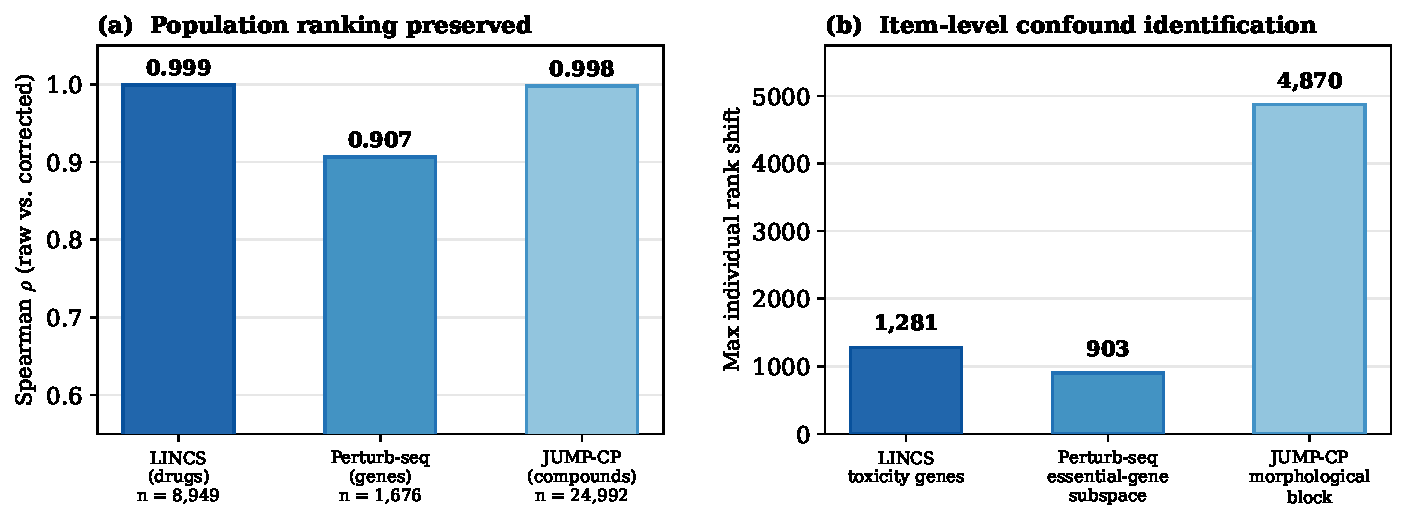
\includegraphics[width=\linewidth]{figures/fig6_cross_domain_empirical.pdf}
\caption{%
\textbf{Cross-domain empirical summary.}
\textbf{(a)}~Spearman $\rho$ between raw and corrected scores in each
domain. All exceed $\rho = 0.90$, so none of the corrections reorganizes
the population ranking. Sample sizes shown below each bar.
\textbf{(b)}~Maximum individual rank shift per domain, showing that
rank-preserving corrections still move specific items. In JUMP-CP the
median absolute percentile-rank shift is 1.0 point and 2.2\% of compounds
move more than five, against a population $\rho = 0.998$.}
\label{fig:cross_domain}
\end{figure}

The same geometric functional---angular deviation of perturbation-response
directions across contexts---applies in all three domains, but its estimand
depends on the context axis (Table~\ref{tab:cross_domain}). In LINCS and
Perturb-seq the axis is biological, so $D$ indexes response consistency
across cell lines and across cell types. In JUMP-CP the axis is the imaging
source, so $D$ indexes technical reproducibility between sites. What the three
share is that deleting the candidate nuisance dimensions preserves the
global ranking. Item-level interpretation rests on an external criterion,
which is available in the two transcriptomic domains and not in JUMP-CP.

\begin{table}[t]
\centering
\caption{Ablation sensitivity by domain. The table compares how much each
feature or gene removal moves the population ranking; it does not assert that
one construct is measured in all three. $^{\dagger}$JUMP-CP is an unregistered
sensitivity analysis whose context axis is the imaging source, so its $\rho$
concerns cross-site technical reproducibility rather than biological
context-dependence. The HDAC calibration panel is omitted
because the threshold was set from it. The LINCS HDAC gradient $\rho$
measures fine-grained ordering within a single drug class (6 compounds
in the selectivity gradient, Figure~\ref{fig:hdac});
the global 8{,}949-drug $\rho > 0.99$. H5 (transport stability) tests
predictive validity rather than rank preservation; the 66-fold
leave-one-out result (Table~\ref{tab:scorecard}) provides the strongest
domain-specific evidence for LINCS.}
\label{tab:cross_domain}
\small
\begin{tabular}{llrl}
\toprule
Domain & Correction & $N$ & $\rho$ \\
\midrule
LINCS (global) & Toxicity genes & 8{,}949 & $>$0.99 \\
Perturb-seq & Essential-gene subspace & 1{,}676 & 0.91 \\
JUMP-CP$^{\dagger}$ & Morphological block & 24{,}992 & 0.998 \\
\bottomrule
\end{tabular}
\end{table}

The domain-specific failure modes differ: in drugs, cytotoxicity
produces high-instability signatures; in genetics, universal-essential
knockdowns produce high-distance subspaces (divergent lethal programs);
in morphology, the ablated block accounts for little of the
between-source directional variance. Each inverts the naive prediction that
``violence mimics transport.''

\subsection{Generalizability of the validation procedure}

The validation framework was tested on one geometric perturbation score
(direction instability) across three biological domains. The
\emph{procedure}---define interpretive threats, specify corrections
that target each threat, pre-register predictions about whether
corrections reorganize rankings, test empirically---applies to other
geometric scores that measure perturbation-response consistency, such as
connectivity scores \citep{subramanian2017next}, morphological similarity
indices, and Grassmannian distance metrics. What would change are the
domain-specific conditions: a connectivity score would require different
confound corrections than direction instability, but the same
structure of threat identification, correction, and pre-registered
testing applies. The effect size for phenotype projection ($\rho = 0.38$,
explaining ${\sim}14\%$ of variance) is moderate. For comparison,
connectivity-score benchmarks in LINCS typically report Spearman
correlations of $\rho = 0.2$--$0.4$ between metric and biological
outcome \citep{li2020comprehensive}, placing the phenotype-projection
result at the upper end of the range achievable with unsupervised
geometric scores on transcriptomic data.

\subsection{Scope and limitations}

Direction instability measures angular consistency of perturbation signatures
across contexts. It does not measure therapeutic efficacy, in-vivo
translatability, or clinical specificity. The validation framework is a
validation framework for perturbation-score interpretation, not a surrogate
endpoint. The consequential validity facet (whether confidence upgrades
change practitioner decisions) is illustrated via the daunorubicin/MG-132
case study but is not empirically tested; a user study or
decision-simulation experiment would be needed to validate this facet.

The drug experiments H3--H5 depend on shRNA knockdown signatures as
ground-truth on-target directions. shRNA has well-documented off-target
effects, which add noise to the ground truth. A CRISPRi
convergent-validity check did not
independently confirm the phenotype-projection result ($\rho = -0.12$,
$p = 0.16$, $n = 131$); the matched 114-drug comparison (shRNA
$\rho = 0.42$ vs.\ CRISPRi $\rho = -0.14$) points to the
pre-registered K562-only confound (CRISPRi signatures from a single
cell type are poor on-target directions for drugs acting in
non-hematopoietic contexts). The shRNA H3 result stands on its original evidence without
independent reinforcement. Drugs with unannotated targets
(7{,}398 of 8{,}949) are excluded from H3 and H4, limiting these conditions
to 17\% of the dataset. LINCS measures 978 landmark genes, restricting
the toxicity gene set to the landmark panel.

The Perturb-seq analysis uses $K = 2$ cell types, providing no Fr\'echet
variance, holonomy, or transport stability test. Both screens target
DepMap-essential genes, so the HP3 ``non-essential'' group consists of
sub-threshold essentials rather than genuinely non-essential genes. A
genome-wide screen with genuine non-essential controls would be sharper,
though the label-permutation null rules out the library-overlap confound.

The transport-stable formula (Eq.~\ref{eq:ts}) is a heuristic
linear combination of direction instability and Fr\'echet variance, not a
principled geometric operation on the signature manifold. The penalty
weight $\lambda = 1.0$ was inherited from the companion paper
\citep{tower2026drug} and was not optimized for this evaluation. A pre-registered sensitivity
analysis across $\lambda \in [0.25, 5.0]$ found the registered win
criterion met more often at larger $\lambda$. Because that criterion
compares signed correlations between oppositely-oriented statistics
(Deviation~6), the pattern reflects the orientation of the penalized score
rather than its predictive value, and is not evidence of robustness.
A ratio or a geodesic-based combination might perform differently.
The simplicity of the linear combination is intentional: it admits
straightforward interpretation of the penalty weight.

A pre-registered dose-direction stability test (6{,}169
drug$\times$cell-line pairs) produced low within-pair cosines (median
0.19; 86.5\% below 0.5), failing both pre-registered criteria. Post-hoc
analysis revealed this failure is dominated by signature-level noise:
80\% of dose-level groups contain a single replicate, and
near-identical doses (ratio $< 1.01$) yield median cosine = 0.11,
establishing a noise floor close to the overall result. The test lacks
statistical power to distinguish genuine dose-dependent direction
changes from single-replicate noise in 978 dimensions. No a priori
power analysis preceded the pre-registration; replicate depth should
have been assessed before committing to specific thresholds.
Direction instability operates at a fixed dose across cell lines, a
regime where the relevant separability condition---that cell-line
response magnitude does not affect direction---is weaker than
dose-independence and holds trivially. The stronger claim (direction
independent of dose) remains empirically unresolved.

LINCS L1000 profiles have known batch effects across plates and
production sites. Batch-driven systematic direction differences would
inflate direction instability for drugs profiled across batches,
producing a confound not addressed by any validity condition tested here.

Deviation entry~1 (Table~\ref{tab:deviations}) documents that the
original pre-registration freeze omitted gene-set construction parameters;
these were specified in the extended pre-registration. The gap between
freezes created a potential researcher degree of freedom in gene-set
construction, partially mitigated by the empirical construction (shRNA
consensus from the same platform requires no pathway-database selection).

The Perturb-seq subspace dimension ($k = 5$) was fixed; geodesic
distances depend on this choice, and a principled selection criterion
(such as an explained-variance threshold) would strengthen the analysis.

The validation framework draws an analogy to Bradford Hill criteria for causal
inference \citep{hill1965environment}. These criteria are individually
neither necessary nor
sufficient for establishing causation; they are heuristic guidelines. The
validation framework shares this character: it is a structured set of proof
obligations rather than a formal deductive system. Each condition eliminates
a specific threat, but satisfying all tested conditions does not
\emph{guarantee} that a mechanistic claim is correct---it guarantees
that specific alternatives have been ruled out.

The JUMP-CP block was defined by substring matching on CellProfiler names
rather than by correlation with an independent viability assay, so it is a
morphological feature family and not a validated cell-health signature; the
analysis therefore does not establish or remove a cell-health confound. Its
size-matched null samples individual columns uniformly, so the block's larger
effect may partly reflect correlation among jointly removed families. The
cohort is also nearly disjoint from PRISM-annotated compound space: 11 of
24{,}992 compounds map uniquely, which precludes validating an item-level
cytotoxicity reading of the rank shifts. The 78.4\% attrition biases the
retained set toward well-replicated compounds.

\section{Conclusions}

Direction instability predicts held-out cell-line agreement in all 66
leave-one-out folds (mean $\rho = -0.602$); a variance-regularized variant
does not improve on it.
Phenotype projection separates on-target from off-target consistency
($\rho = 0.38$ vs.\ $-0.04$). Essential-gene correction identifies
proteasome/spliceosome genes as confound-dominated while preserving the
population ranking ($\rho = 0.91$). These results hold across three
perturbation domains---8{,}949 LINCS drugs, 1{,}676 Perturb-seq
knockdowns, 24{,}992 JUMP-CP compounds---with domain-specific failure
modes that invert naive predictions in each case.

The validation framework tested here---define confounds, specify
corrections, pre-register predictions, test whether corrections reorganize
rankings or preserve them---applies to any geometric score measuring
perturbation-response consistency across contexts. Localization helps for
intracellular enzyme targets but not receptor-mediated drugs, constraining
where specific conditions apply. The domain-specific corrections differ,
but the pattern is the same: correction preserves population rankings while
identifying individual perturbations most susceptible to confounding. The
framework provides a structured, pre-registerable procedure for diagnosing
which confounds a geometric perturbation score has survived.

\section*{List of abbreviations}
AUROC: area under the receiver operating characteristic curve;
CRISPRi: CRISPR interference;
DI: direction instability;
GO: Gene Ontology;
HDAC: histone deacetylase;
JUMP-CP: Joint Undertaking for Morphological Profiling -- Cell Painting;
LINCS: Library of Integrated Network-Based Cellular Signatures;
LOO: leave-one-out;
MOA: mechanism of action;
PCA: principal component analysis;
shRNA: short hairpin RNA;
TS: transport-stable (variance-regularized) direction instability.

\section*{Declarations}

\subsection*{Ethics approval and consent to participate}
Not applicable. This study uses only publicly available datasets
(LINCS L1000, Perturb-seq, JUMP-CP, DepMap) with no human subjects
research.

\subsection*{Consent for publication}
Not applicable.

\subsection*{Availability of data and materials}
All data used in this study are publicly available: LINCS L1000
(GEO GSE92742), Perturb-seq \citep{replogle2022mapping}, JUMP-CP
\citep{chandrasekaran2023jump}, DepMap \citep{dempster2021chronos}.
Code, pre-registration commits (SHA \texttt{8d74bd0} for initial
freeze; SHA \texttt{f3c88ed}, tag \texttt{prereg-extended-psb}, for
extended pre-registration; SHA \texttt{5bb6080} for dose-direction
separability test), deviation log, and all experimental scripts are
available at
\url{https://github.com/elliottower/direction-instability-drug-validity}.
The repository was public before the pre-registration freeze.
A permanent archive is deposited at Zenodo
(DOI: \url{https://doi.org/10.5281/zenodo.21284088}).

\subsection*{Competing interests}
The author declares no competing interests.

\subsection*{Funding}
This work received no external funding.

\subsection*{Authors' contributions}
ET conceived the study, designed the validation framework, conducted
all experiments, and wrote the manuscript.

\subsection*{Use of AI-assisted technologies}
Claude (Anthropic) was used as a writing and analysis assistant during
manuscript preparation. The author directed all analytical decisions and
verified all numerical results against source data. The validation framework,
pre-registered hypotheses, experimental results, and interpretations are
the author's own. The author takes full responsibility for the content.
No AI tool is listed as an author.

\subsection*{Acknowledgements}
Not applicable.

\subsection*{Supplementary information}
Additional file 1: Supplementary Experiments and Extended Results.
Full methods, tables, and discussion for Experiments~1, 2, and~4
(H1 toxicity correction, H2 broad-mechanism drugs, H4 localization
score) and HP2 (GO pathway prediction from corrected Perturb-seq
distances). Includes the complete HDAC drug list used in the
sensitivity analysis and Supplementary Table~S1 (Messick validity-facet
mapping).

\bibliographystyle{unsrtnat}
\bibliography{references}

\end{document}
